\documentclass{standalone}
\usepackage{pgfplots}
\begin{document}
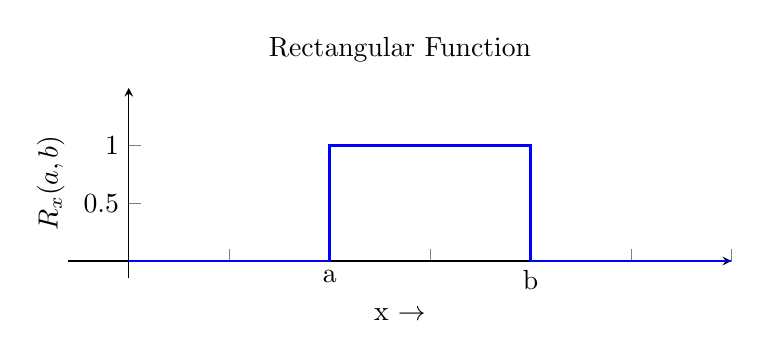
\begin{tikzpicture}
\begin{axis}[
width=10cm,
height=4cm,
x axis line style={-stealth},
y axis line style={-stealth},
title={Rectangular Function},
xticklabels={0,,,a,,b},
ymax = 1.5,xmax=3,
axis lines*=center,
ytick={0.5,1},
xlabel={x $\rightarrow$},
ylabel={$R_x(a,b)$},
xlabel near ticks,
ylabel near ticks]
\addplot+[thick,mark=none,const plot]
coordinates
{(0,0) (1,0) (1,1) (2,0) (3,0) (4,1) (5,0) (6,1) (7,0)};
\end{axis}
\end{tikzpicture}

\end{document}